% !TEX root = master.tex

We have developed techniques for automated sky analysis, bulge+disc fitting and truncation characterisation. We have compiled truncation parameters for a large sample of galaxies and investigated their correlations cluster environment. 

\subsection{Comparison with previous studies}
There is one type-II in our study, making up just under 2\% of our sample. This is consistent with the findings of \citet{erwin_strong_2012} in that there are very few if not any disks which exhibit downbending in the cluster environment. 
\begin{figure}
	\centering
	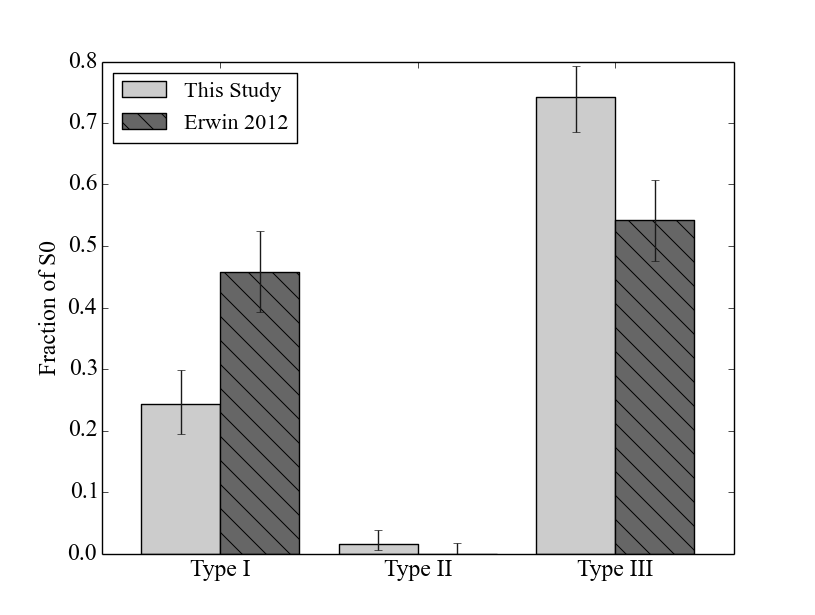
\includegraphics[width=\textwidth]{figs/total_bar_chart_truncs.png}
	\caption{Comparison of Type fraction in the Coma cluster to Virgo \citep{erwin_strong_2012}. Error bars show 68\% confidence intervals \citep{wilson_probable_1927}}
\end{figure}
However, our study finds that there is a greater divide between Type-Is and Type-IIIs with 24\% and 74\% respectively. The frequency of type-I S0s appears not to be dependent on environment. This suggests 


\subsection{Problems with this method}
Fitting in 1D is swift and easier than a full 2D decomposition. However, neglecting most of the light of the galaxy impacts on the accuracy of the profile fitted. Any perturbation or artefact -such as a bar or flat-fielding error- included in the major axis wedge cannot be easily or safely removed. Therefore, the two major axis profiles will strongly disagree if there is a slight difference between them. Further problems arise from the combination of profiles from different cameras. 

Combining four bootstraps is effective when the individual results are already close to each other (within $\sim 1\sigma$) and a disagreeing fourth may be discarded provided the other three agree. When there is a divide in parameter space larger than $\sim 2\sigma$ the resulting combination will yield a result which neither bootstrap group supports and with large errors. 

Sky detection has worked effectively in this investigation but whether our values are correct or not is untestable until there are more readings around the galaxy in addition to those at the end of the major-axis. 